\section{(2) Kontextualisierung des Prototyps und Reflektion}\label{kontextualisierung}

Die Installation fand statt am 05. Februar 2025, von 13:30 Uhr bis 16:00 Uhr am Stadt:Raum Bamberg, direkt am zentralen Omnibusbahnhof der Stadt.
Zuvor bauten wir die Installation vor Ort rund 20 Minuten öffentlich
auf.
Kurz nachdem wir die Installation der Öffentlichkeit überließen und uns zurückzogen, interagierten die ersten zwei Passanten, indem sie eine Partei wählten.
Vermutlich hat der beobachtbare öffentliche Aufbau der Wahlkabine dazu beigetragen, dass sich die ersten beiden Interaktionen unmittelbar ereigneten, wohingegen die übrigen Interaktionen zeitlich deutlich entzerrter sind.

\subsection{Publikum}\label{publikum}

Das Publikum am zentralen Omnibusbahnhof bestand im Wesentlichen aus zwei Gruppen.

Eine Gruppe umfasst die Personen, die wartend an einer Haltestelle auf der ZOB-Insel standen und Blick auf die Installation hatten. Dies waren ab 13:30 Uhr mehrheitlich Schüler.
Zu diesem Zeitpunkt war der ZOB gut gefüllt.
Ab ca. 14:30 Uhr hielten sich hingegen nur noch wenige Passanten an den Haltestellen auf.

Die zweite Gruppe besteht aus Passanten, die zufällig direkt an der Installation vorbeiliefen; mehrheitlich Personen im Alter ab ca. 40 Jahren.

Im Zeitraum von 13:55 Uhr bis 15:05 dokumentierten wir den Durchgangsverkehr vor der Installation, das Verhalten der Passanten und die jeweilige Gruppengröße.
Insgesamt kamen in den 70 Minuten 145 Personen direkt an der Installation vorbei.
112 gingen ohne Reaktion weiter, 31 Personen schauten auf das Display oder in die Wahlkabine (ohne zu Wählen) und 2 Personen gaben jeweils einzeln und unabhängig von einander ihre Stimme ab.
Unter den 145 Personen befanden sich 24 Gruppen á 2 Personen.

\subsubsection{Aktivierungsmuster}\label{aktivierungsmuster}

Während des Experiments fielen uns drei Muster auf, wie Passanten auf die Installation aufmerksam wurden.
Bis auf eine einzige Person haben alle interagierenden Passanten gemeinsam, dass sie nur deshalb interagierten, weil sie auf ihrem Weg sowieso an der Installation vorbeigehen mussten und somit zufällig auf die Wahlkabine oder Display 1
aufmerksam wurden.
Nur eine einzige Person querte zielgerichtet die Straße und wich somit von ihrem eigentlichen Weg ab, um zu partizipieren.

\paragraph{Muster 1: Vorbeigehen \& Schauen}
Das häufigste Interaktionsmuster bestand darin, dass Passanten, die den Gehsteig vor dem Stadt:Raum entlangliefen, die Ergebnisse auf Display 1 betrachteten oder die Wahlkabine beim Vorbeigehen kurz in Augenschein nahmen.
Display 1, dass die Wahlumfrageergebnisse zeigte, verleitete damit Passanten dazu, anzuhalten und sich die Ergebnisse einen Moment anzusehen, bevor sie weitergingen.
Die Wahlkabine diente in diesem Fall als Trigger, der die Aufmerksamkeit auf den Stadt:Raum zog und dadurch womöglich die Wahrnehmung von Display 1 förderte.
Nur wenige Passanten blieben stehen, um die Wahlkabine genauer anzusehen, sondern widmeten ihr im Vorbeigehen ein paar Blicke.
Drei Passanten betraten zwar die Wahlkabine, wählten aber nicht.
Der Großteil der Passanten hat natürlicherweise weder Display 1, noch der Wahlkabine ihre Aufmerksamkeit geschenkt.

\paragraph{Muster 2: Vorbeigehen \& Wählen}
Alle Wähler, bis auf Einen, kamen zufällig an der Wahlkabine vorbei und interagierten infolge dessen.
Keiner der Wähler hat nachträglich auf dem benachbarten Display 1 nachgesehen, wie die Verteilung der Gesamtstimmen ausfällt.
Die Wähler waren alle männlich und mehrheitlich vermutlich über 40 Jahre alt.

\paragraph{Muster 3: Straße queren}
Ein Passant (männlich, ca. 18 Jahre alt) querte vor der Interaktion aktiv die Straße und betrachtete auf Display 1 die Gesamtverteilung der Stimmen.
Er fotografierte das Display mit seinem Smartphone und betrat daraufhin die Wahlkabine, um seine Stimme abzugeben.
Da sich die Wahlentscheidung des jungen Manns mit der Partei mit den zu dieser Zeit meisten Stimmen deckte, mutmaßen wir, dass die Umfrageergebnisse ihn dazu motiviert haben, selbst abzustimmen.


\subsubsection{Interaktion}\label{interaktion}

Während des Deployments waren gleichermaßen vollständig durchgeführte Wahl-Interaktionen (Stimmabgabe ist erfolgt) und unvollständige Wahl-Interaktionen (es wurde versucht, eine Stimme abzugeben, aber es gelang nicht) zu beobachten.

Zwei Seniorinnen hielten sich unabhängig von einander für eine Zeit von 30 bis 60 Sekunden in der Wahlkabine auf, ohne dass eine Stimmabgabe erfasst wurde.
Bei einer der beiden Damen war zu beobachten, dass sie sogar in den Korb mit den Wahlkarten griff.
In Folge dessen war für sie entweder unklar, was sie mit den Wahlkarten tun kann oder sie entschloss sich, nicht zu wählen, weil ihre Partei nicht als Wahlkarte abgebildet war (nur als Option ``Sonstige'').

Ein weiterer Passant (ca. Mitte 40) sprach uns aktiv an, als wir uns gerade in der Nähe der Wahlkabine befanden und fragte, ob er dort seine Stimme für die Bundestagswahl abgeben könne.
Nachdem wir ihm das Experiment erklärt hatten, entschloss sich der Mann, an der Umfrage teilzunehmen.
Er löste die mit einer Schnur an der Installation befestigte Wahlkarte (die Befestigung diente dazu, Diebstahl zu verhindern und sollte gleichzeitig verdeutlichen, dass die Wahlkarte wieder zurückzulegen und nicht einzuwerfen ist) und fragte uns, was damit zu tun ist.
Nachdem wir dem Mann das System erklärt hatten, steckte er die Wahlkarte mehrmals hektisch falsch herum in die Wahlurne und war sich im Unklaren darüber, ob seine Stimme erfasst wurde oder nicht.
Der Mann blickte dabei nicht auf das Display, sondern herunter auf die Wahlurne und konnte so auch nach erfolgreicher Stimmabgabe nicht feststellen, dass seine Stimme registriert wurde.
Wir mutmaßen, dass der Mann das Display vollständig ignorierte, weil er glaubte, bereits alle Informationen von uns erhalten zu haben.
Zudem betonte er mehrmals, dass er sehr in Eile ist (der Mann trug erkennbare Arbeitskleidung).
Auch deshalb hat er sich wahrscheinlich nicht noch einmal die Zeit genommen, die Informationen auf dem Display zu lesen.

Um die Interaktion für die ersten Interessenten zu erleichtern, haben wir am Anfang bereits 10 Stimmen hinzugefügt.
Diese waren zufällig, aber entsprechend der Verteilung der damals aktuellen Umfrageergebnisse, gewählt.
Die folgenden Abbildungen zeigen die abgegebenen Stimmen im Zeitverlauf und das Ergebnisse.
Das unbereinigte Ergebnisse entspricht dem, was am Schluss auf Display 1 zu sehen war, und enthält neben den Seed-Daten auch 2 Instanzen von doppelter Stimmabgabe, bei denen jeweils weniger als 10 Sekunden seit der vorhergehenden Teilnahme vergangen waren.
Zusätzlich waren darin Stimmen enthalten, die wir selbst zur Aufzeichnung unseres Videos abgegeben haben.
All diese Stimmen wurden aus dem bereinigten Ergebnis entfernt, das in Abbildung \ref{fig:result-cleaned} zu sehen ist.

\begin{figure}[ht]
    \centering
    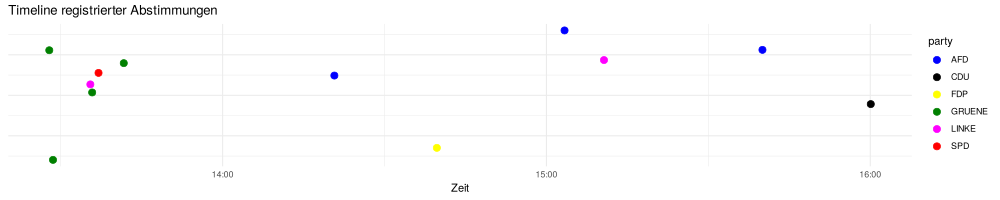
\includegraphics[width=0.8\textwidth]{figures/timeline-cleaned.pdf}
    \caption{Timeline der Interaktionen (bereinigt, siehe Abbildung \ref{fig:result-cleaned})}
    \label{fig:timeline}
\end{figure}

\begin{figure}[ht]
    \centering
    \begin{minipage}{.48\textwidth}
        \centering
        \includegraphics[width=.9\linewidth]{figures/result-all.pdf}
        \captionof{figure}{Abstimmungsergebnis, wie am Ende des Experiments zu sehen}
        \label{fig:result-all}
    \end{minipage}%
    \begin{minipage}{.48\textwidth}
        \centering
        \includegraphics[width=.9\linewidth]{figures/result-cleaned.pdf}
        \captionof{figure}{Abstimmungsergebnis, bereinigt}
        \label{fig:result-cleaned}
    \end{minipage}
\end{figure}
\subsection{Raumtypen}\label{raumtypen}

\subsubsection{Display Space}\label{display-space}

Im markierten Display Space sind nicht aus jeder Position beide Displays sichtbar, aus bestimmten Positionen ist sogar gar kein Display sichtbar.
Allerdings ist mindestens die Wahlkabine aus jeder Position sichtbar, weshalb wir den Display Space entsprechend groß gewählt haben.
Angrenzend an den Display Space befindet sich der Activation Space (nicht extra eingezeichnet), an dem Passanten auf die Installation aufmerksam werden /könnten/.

\subsubsection{Interaction Space}\label{interaction-space}

Der Interaction Space befand sich unmittelbar vor Display 1 und in der Wahlkabine.
Durch die Wahlkabine war der Interaction Space an dieser Stelle sehr isoliert, wohingegen der Interaction Space vor Display 1 auch Potential für Gruppeninteraktionen bot.
In der Praxis hat sich gezeigt, dass auch Gruppen aus zwei Personen gemeinsam vor Display 1 stehen blieben und über die Ergebnisse sprachen.

\subsubsection{Gap Space}\label{gap-space}

Aufgrund der Beschaffenheit des ZOB entstand durch die von Bussen befahrene Straße zwischen Gehsteig und Haltestellen ein toter Raum, der Distanz zur Installation schaffte.
Insbesondere wenn ein Bus für mehrere Minuten an einer Haltestelle stand und die Sicht auf die Installation verdeckte, war der Raum hinter dem Bus verloren.

\subsubsection{Comfort Space}\label{comfort-space}

Kurz hinter dem Gap Space befinden sich mehrere Sitzgelegenheiten an den Haltestellen, die Comfort Spaces bilden.
Von hier aus ist das Geschehen an der Installation beim Warten auf den Bus direkt beobachtbar.
Der mittlere Comfortspace ist der Interessanteste, da von hier aus sowohl die Wahlkabine als auch Display 1 eingesehen werden können.
Wir nahmen an, dass an dieser Stelle auch ein Social Interaction Space entstehen könnte, indem das Beobachtete in Gruppen zum Gesprächsthema wird und daraus neue Trigger zur Interaktion mit der Installation entstehen.
Dies konnten wir leider nicht beobachten.
Das Queren der Straße zum Abgeben der Stimme war der Ausnahmefall.
\subsection{Verbesserungspotenzial}\label{verbesserungspotenzial}

Das Experiment hat gezeigt, dass die Installation die beabsichtigten Interaktionen triggern und von Passanten verstanden werden kann.
Es gab jedoch auch Passanten, die nicht wussten, was sie tun sollten.
Einzelne Teilaspekte des Konzepts gingen zudem nicht vollständig auf.
Es stellte sich heraus, dass der wahrnehmbare Zusammenhang der beiden Displays sowie die Displayinhalte nicht optimal gelöst waren.
Auch das User-Feedback an der Wahlkabine ließe sich verbessern.

\subsubsection{Zusammengehörigkeit der Displays}\label{zusammenhang-der-displays}

Während des Experiments hat sich herausgestellt, dass der Zusammenhang der beiden Displays vermutlich nicht für alle ersichtlich war.
Passanten wählten, ohne sich vor oder nach ihrer Wahl das nur wenige Meter entfernte Display mit den Umfrageergebnissen anzusehen.
Gleichermaßen haben Personen, die sich interessiert die Ergebnisse angesehen haben, nicht an der Wahl teilgenommen.

Wir gingen davon aus, dass die Einsicht in die Abstimmungsergebnisse als Trigger dienen kann.
Einerseits, indem man seine Wahlpräferenz unterrepräsentiert sieht und der Partei infolge dessen zu mehr Stimmen verhelfen möchte.
Andererseits, indem man seine Partei gut performen sieht und dementsprechend noch eine weitere Stimme zur Unterstützung gibt.
Ein Mann (ungefähr 50 Jahre alt) schaute im Abstand einiger Zeit sogar zweimal auf die Umfrageergebnisse auf Display 1 und zeigte durch Kopfschütteln eine Reaktion auf die Ergebnisse.
Er gab seine eigene Stimme jedoch nicht ab.

Deshalb hätte auf beiden Displays klarer darauf hingewiesen werden müssen, dass noch ein weiteres Display existiert.
Die Information war zwar in Textform vorhanden, ging aber offenbar auf dem Display unter.
Hierzu sollten die Displayinhalte überarbeitet werden.

\subsubsection{Displayinhalte}\label{displayinhalte}

Die beiden Displays waren weitestgehend statisch und veränderten sich nur dann in Teilen, wenn eine Stimmabgabe registriert wurde.
Statische Displays ziehen bei Weitem nicht so viel Aufmerksamkeit auf sich, wie bewegte Inhalte.
Das wurde uns während des Experiments sehr deutlich klar, da Display 2 (vor der Wahlkabine) durch einen technischen Defekt ungefähr einmal pro Minute kurz aus- und wieder anflackerte, was automatisch den Blick dorthin wandern ließ, wenn sich das Display im Sichtfeld befand.

Anstatt alle Informationen auf einer Seite anzuordnen, hätte man sie dynamisch nacheinander anzeigen lassen können - mit Animationen, die die Aufmerksamkeit auf sich ziehen.
Dadurch wäre es auch möglich gewesen, den Displayzusammenhang zu verdeutlichen.

Für Display 2 in der Wahlkabine stellte sich heraus, dass durch die sehr nahe Platzierung der Wahlkabine am Schaufenster das Sichtfeld eingeschränkt wurde.
Das Display war nicht vollständig wahrnehmbar, ohne seinen Kopf zu bewegen.
Der Blick fiel somit immer nur auf einen Teilbereich des Displays, wohingegen die Bereiche drum herum währenddessen auch aus dem peripheren Sichtfeld verschwanden und damit blind waren.
Zwar testeten wir die Anzeige vorher, doch ohne dazu die Wahlkabine aufzustellen, da diese durch ihre Größe etwas schwierig zu transportieren ist.
Ein Test mit Wahlkabine hätte dieses Problemfeld früher aufzeigen können.

\subsubsection{User-Feedback während der Wahl-Interaktion}\label{user-feedback-bei-der-wahl-interaktion}

Während des Experiments ist aufgefallen, dass Teilnehmer, die das System nicht kennen, beim Wählen nach unten auf die Wahlurne blicken und nicht geradeaus auf das Display.
Ein zusätzliches Feedback als Erfolgsindikator, etwa ein Ton oder ein Leuchtsignal direkt an der Wahlurne, könnte das Verständnis erleichtern.

\subsection{Öffentlichkeit der Wahl}\label{uxf6ffentlichkeit-der-wahl}

Wohl auch bedingt durch die bereits beschriebene Tatsache, dass den Teilnehmenden augenscheinlich die Verbindung zwischen den beiden Displays nicht ausreichend klar war, gab es keinerlei Reaktion auf die Öffentlichkeit der Wahl.
Von Passanten, die nicht aktiv an der Wahl teilnahmen, gab es zwar Reaktionen auf die Wahlergebnisse, nicht aber auf konkrete Stimmabgaben.
